\subsubsection{Onset of convection benchmark}
\label{sec:benchmark-onset-of-convection}
\textit{This section was contributed by Max Rudolph, based on a course assignment for ``Geodynamic Modeling'' at Portland State University.}

Here we use \aspect{} to numerically reproduce the results of a linear stability analysis for the onset of convection in a fluid layer heated from below. This exercise was assigned to students at Portland State University as a first step towards setting up a nominally Earth-like mantle convection model. Hence, representative length scales and transport properties for Earth are used. This cookbook consists of a jupyter notebook (\texttt{benchmarks/onset-of-convection/onset-of-convection.ipynb}) that is used to run \aspect{} and analyze the results of several calculations. To use this code, you must compile \aspect{} and give the path to the executable in the notebook as \texttt{aspect\_bin}.

The linear stability analysis for the onset of convection appears in Turcotte and Schubert \cite{TS14} (section 6.19). The linear stability analysis assumes the Boussinesq approximation and makes predictions for the growth rate (vertical velocity) of instabilities and the critical Rayleigh number $Ra_c$ above which convection will occur. $Ra_c$ depends only on the dimensionless wavelength of the perturbation, which is assumed to be equal to the width of the domain. The domain has height $b$ and width $\lambda$ and the perturbation is described by
\begin{align*}
T'(x,y) = T_0'\cos\left(\frac{2\pi x}{\lambda}\right)\sin\left(\frac{\pi y}{b} \right),
\end{align*}
where $T_0'$ is the amplitude of the perturbation. Note that because we place the bottom boundary of the domain at $y=0$ and the top at $y=b$, the perturbation vanishes at the top and bottom boundaries. This departs slightly from the setup in \cite{TS14}, where the top and bottom boundaries of the domain are at $y=\pm b/2$. The analytic expression for the critical Rayleigh number, $Ra_c$ is given in Turcotte and Schubert \cite{TS14} equation (6.319):
\begin{align*}
Ra_c=\frac{\left(\pi^2+\frac{4\pi^2 b^2}{\lambda^2}\right)^3}{\frac{4\pi^2 b^2}{\lambda^2}}.
\end{align*}
The linear stability analysis also makes a prediction for the dimensionless growth rate of the instability $\alpha'$ (Turcotte and Schubert \cite{TS14}, equation (6.315)). The maximum vertical velocity is given by
\begin{align*}
v_{y,\text{max}} = \frac{2\pi}{\lambda}\phi_0' e^{\alpha' t},
\end{align*}
where
\begin{align*}
\phi_0' = -\frac{2\pi}{\lambda}\frac{\rho_0 g \alpha T_0'}{\mu}\left(\frac{4\pi^2}{\lambda^2}+\frac{\pi^2}{b^2} \right)^{-2},
\end{align*}
and
\begin{align*}
\alpha'=\frac{\kappa}{b^2}\left[\frac{\rho_0 g \alpha b^3 \Delta T}{\mu \kappa}\left(\frac{\frac{4\pi^2 b^2}{\lambda^2}}{\left(\frac{4\pi^2 b^2}{\lambda^2}+\pi^2\right)^2}\right) -\left(\pi^2+\frac{4\pi^2b^2}{\lambda^2}\right)\right].
\end{align*}

We use bisection to determine $Ra_c$ for specific choices of the domain geometry, keeping the depth $b$ constant and varying the domain width $\lambda$. If the vertical velocity increases from the first to the second timestep, the system is unstable to convection. Otherwise, it is stable and convection will not occur. Each calculation is terminated after the second timestep. Fig.~\ref{fig:onset-1} shows the numerically-determined threshold for the onset of convection, which can be compared directly with the theoretical prediction (green curve) and Fig.~6.39 of \cite{TS14}. The relative error between the numerically-determined value of $Ra_c$ and the analytic solution are shown in the right panel of Fig.~\ref{fig:onset-1}.

\begin{figure}
 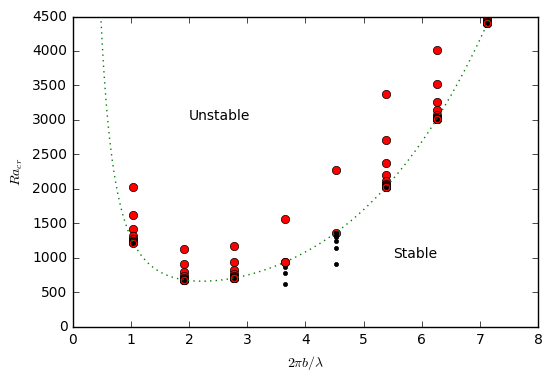
\includegraphics[width=0.49\textwidth]{cookbooks/benchmarks/onset-of-convection/doc/racr.png}
 \hfill
 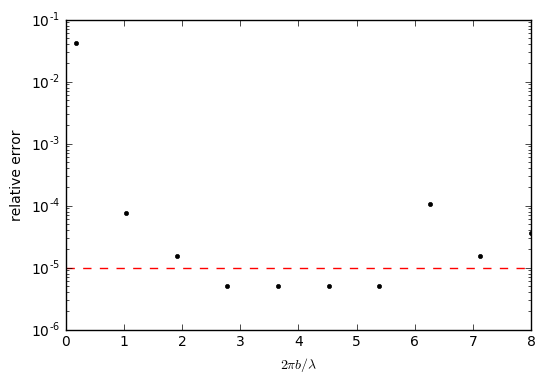
\includegraphics[width=0.49\textwidth]{cookbooks/benchmarks/onset-of-convection/doc/racr_error.png}
 \caption{\it Left: Comparison of numerically-determined and theoretical values for $Ra_c$. Red circles indicate numerical simulations unstable to convection, black circles indicate simulations that are stable. The green dashed curve indicates the theoretical prediction. Right: Relative error in determination of $Ra_c$. The dashed red line indicates the error tolerance used in bisection procedure.}
 \label{fig:onset-1}
\end{figure}


